% \documentclass[aspectratio=169,notes]{beamer}
\documentclass[aspectratio=169]{beamer}
\usetheme[faculty=phil]{fibeamer}
\usepackage{polyglossia}
\setmainlanguage{english} %% main locale instead of `english`, you
%% can typeset the presentation in either Czech or Slovak,
%% respectively.
\setotherlanguages{russian} %% The additional keys allow
%%
%%   \begin{otherlanguage}{czech}   ... \end{otherlanguage}
%%   \begin{otherlanguage}{slovak}  ... \end{otherlanguage}
%%
%% These macros specify information about the presentation
\title[MaM]{Mechanics and Machines, Lecture 8} %% that will be typeset on the
\subtitle{Connections:
\\ Detachable (Threaded, Keyed, Pin, Split pin) \\   
Permanent (Riveting, Welding, Soldering, Glue)} %% title page.
\author{Oleg Bulichev}
%% These additional packages are used within the document:
\usepackage{ragged2e}  % `\justifying` text
\usepackage{booktabs}  % Tables
\usepackage{tabularx}
\usepackage{tikz}      % Diagrams
\usetikzlibrary{calc, shapes, backgrounds}
\usetikzlibrary{decorations.pathreplacing,calligraphy,calc,graphs}
\usepackage{amsmath, amssymb}
\usepackage{url}       % `\url`s
\usepackage{listings}  % Code listings
% \usepackage{subfigure}
\usepackage{floatrow}
\usepackage{subcaption}
\usepackage{mathtools}
\usepackage{todonotes}
\usepackage{fontspec}
\usepackage{multicol}
\usepackage{pdfpages}
\usepackage{wrapfig}
\usepackage{animate}
\usepackage{booktabs}
\usepackage{multirow}
% \usepackage{graphicx}
\usepackage{colortbl}

\graphicspath{{resources/}}
\frenchspacing

\setbeamertemplate{caption}[numbered]
\usetikzlibrary{graphs}

% \usepackage[backend=biber,style=ieee,autocite=footnote]{biblatex}
% \addbibresource{biblio.bib}
% \DefineBibliographyStrings{english}{%
%   bibliography = {References},}

\newcommand{\oleg}[2][] {\todo[color=red, #1] {OLEG:\\ #2}}
\newcommand{\fbckg}[1]{\usebackgroundtemplate{\includegraphics[width=\paperwidth]{#1}}}%frame background

\usepackage[framemethod=TikZ]{mdframed}
\newcommand{\dbox}[1]{
\begin{mdframed}[roundcorner=3pt, backgroundcolor=yellow, linewidth=0]
\vspace{1mm}
{#1}
\vspace{1mm}
\end{mdframed}
}

\begin{document}
\setlength{\abovedisplayskip}{0pt}
\setlength{\belowdisplayskip}{0pt}
\setlength{\abovedisplayshortskip}{0pt}
\setlength{\belowdisplayshortskip}{0pt}

\fbckg{fibeamer/figs/title_page.png}
\frame[c]{\setcounter{framenumber}{0}
    \usebeamerfont{title}%
    \usebeamercolor[fg]{title}%
    \begin{minipage}[b][6.5\baselineskip][b]{\textwidth}%
        \textcolor{black}{\raggedright\inserttitle}
    \end{minipage}
    % \vskip-1.5\baselineskip

    \usebeamerfont{subtitle}%
    \usebeamercolor[fg]{framesubtitle}%
    \begin{minipage}[b][3\baselineskip][b]{\textwidth}
        \raggedright%
        \insertsubtitle%
    \end{minipage}
    \vskip.25\baselineskip
}
%   \frame[c]{\maketitle}

\fbckg{fibeamer/figs/common.png}

\note{\scriptsize \begin{itemize}
        \item \
    \end{itemize}}

\begin{frame}[t]{Connections}
    \framesubtitle{Classification}
    \vspace{-0.7cm}
    \begin{figure}[H]
        \begin{subfigure}{0.48\textwidth}
            \centering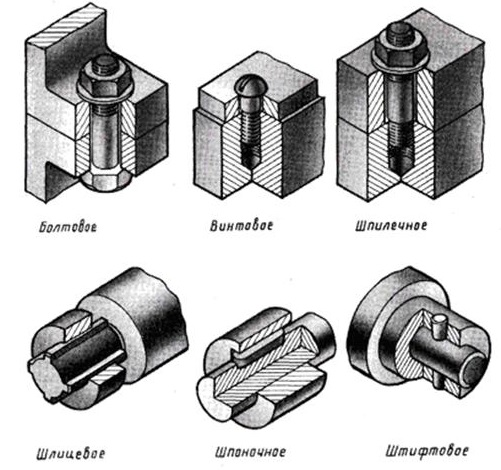
\includegraphics[height=5.5cm,width=1\textwidth,keepaspectratio]{detach.jpg}
            \caption*{Detachable (Разъемные)}
            \label{fig:detach.jpg}
        \end{subfigure}
        \begin{subfigure}{0.48\textwidth}
            \centering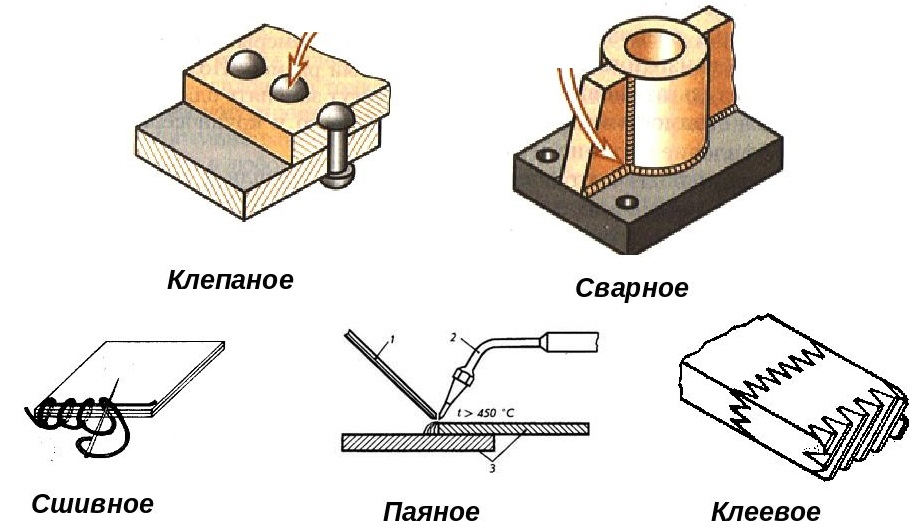
\includegraphics[height=5.5cm,width=1\textwidth,keepaspectratio]{fixed.jpg}
            \caption*{Permanent (Неразъемные)}
            \label{fig:fixed.jpg}
        \end{subfigure}
    \end{figure}
\end{frame}

\begin{frame}[t]{Keyed (шпоночное) and Spline (шлицевое)}
    \framesubtitle{}
    \begin{columns}[T,onlytextwidth]
        \begin{column}{0.49\textwidth}
            They attach, gears, pulleys, and cams on shafts to obtain machinery. In general, we call the assembly sections of these parts shafts hubs.

            So, we use keys in the attachment of these elements to shafts.
        \end{column}
        \begin{column}{0.49\textwidth}
            \begin{figure}[H]
                \centering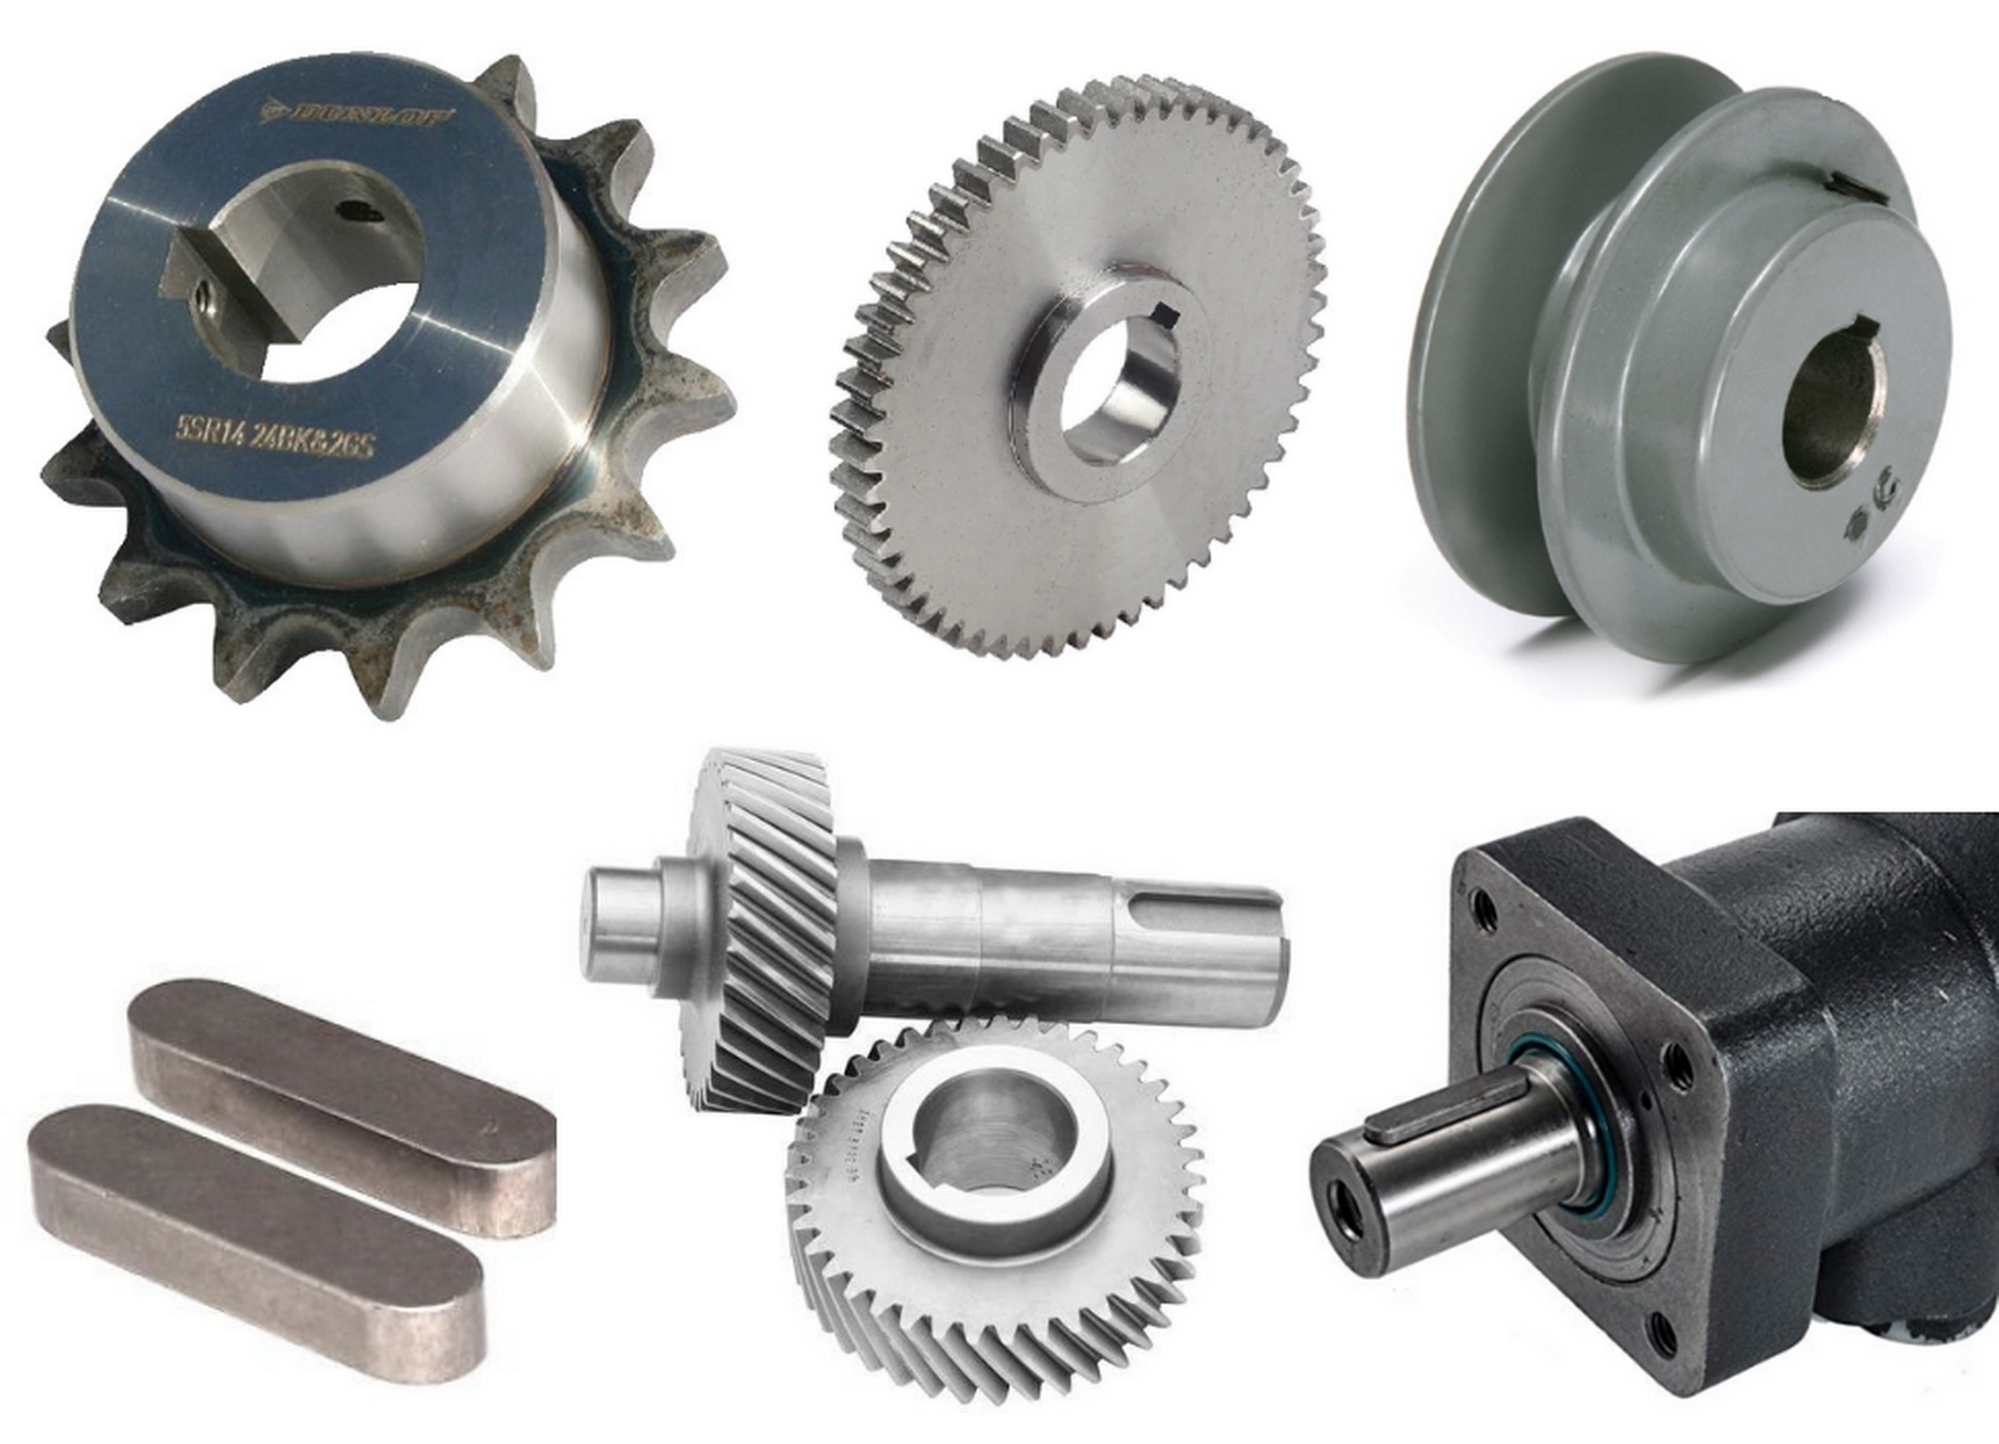
\includegraphics[height=5cm,width=1\textwidth,keepaspectratio]{find_key.png}
                \label{fig:find_key.png}
            \end{figure}
        \end{column}
    \end{columns}
\end{frame}

\begin{frame}[t]{Types of keys}
    \framesubtitle{Video}
    \vspace{-0.6cm}
    \begin{figure}[H]
        \href{https://youtu.be/F3c6GPAFZMI}{
            \centering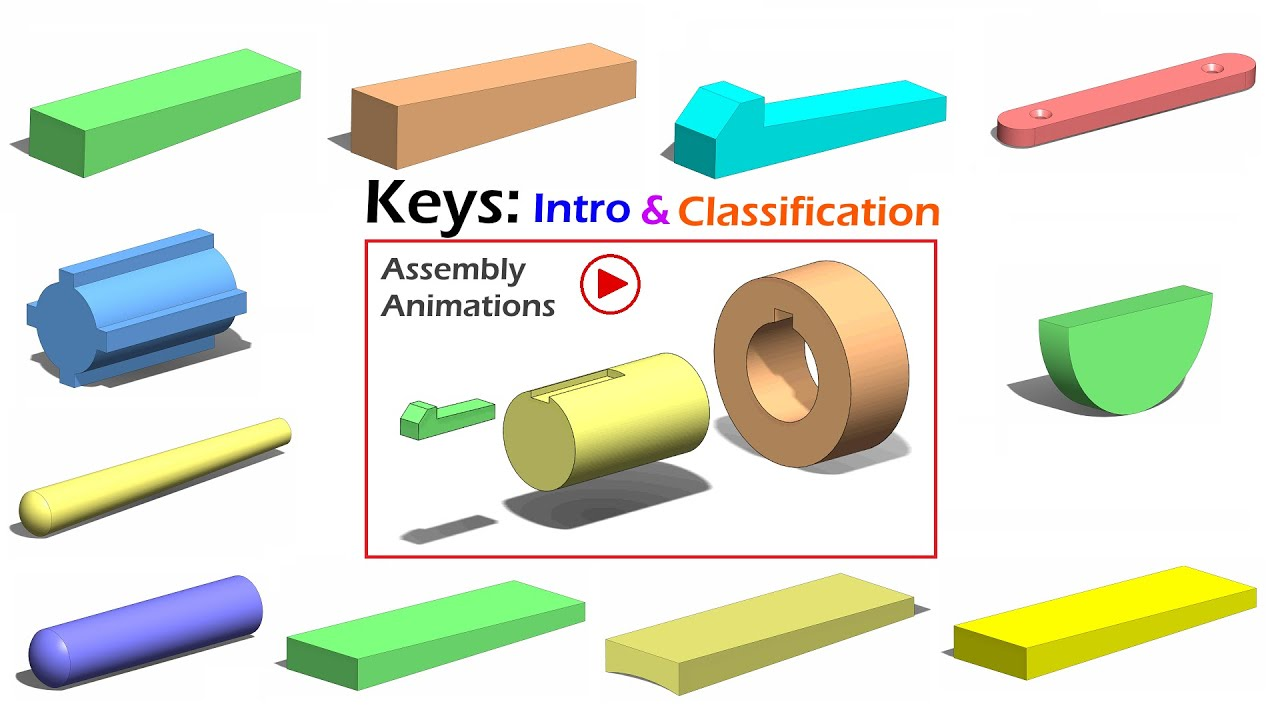
\includegraphics[height=6cm,width=1\textwidth,keepaspectratio]{keyed_video.jpg}}
        \label{fig:keyed_video.jpg}
    \end{figure}
\end{frame}

\begin{frame}[t]{Types of keys}
\framesubtitle{}
    \vspace{-0.6cm}
    \begin{figure}[H]
        \centering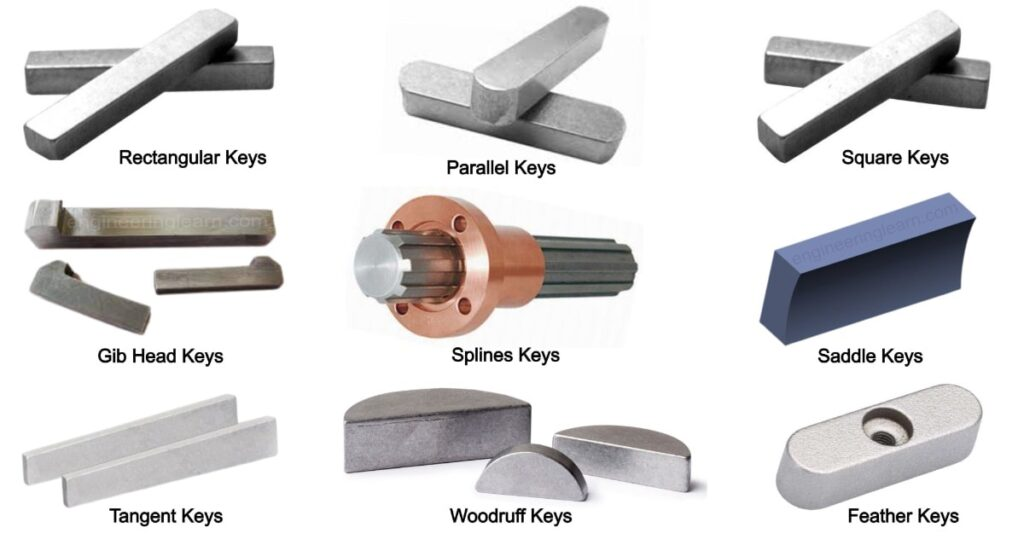
\includegraphics[height=6cm,width=1\textwidth,keepaspectratio]{types_of_keys.jpg}
        \label{fig:types_of_keys.jpg}
    \end{figure}
\end{frame}

\begin{frame}[t]{Keys and splines (rus)}
    \framesubtitle{Video}
    \vspace{-0.6cm}
    \begin{figure}[H]
        \href{https://youtu.be/-bktOSXtLB8}{
            \centering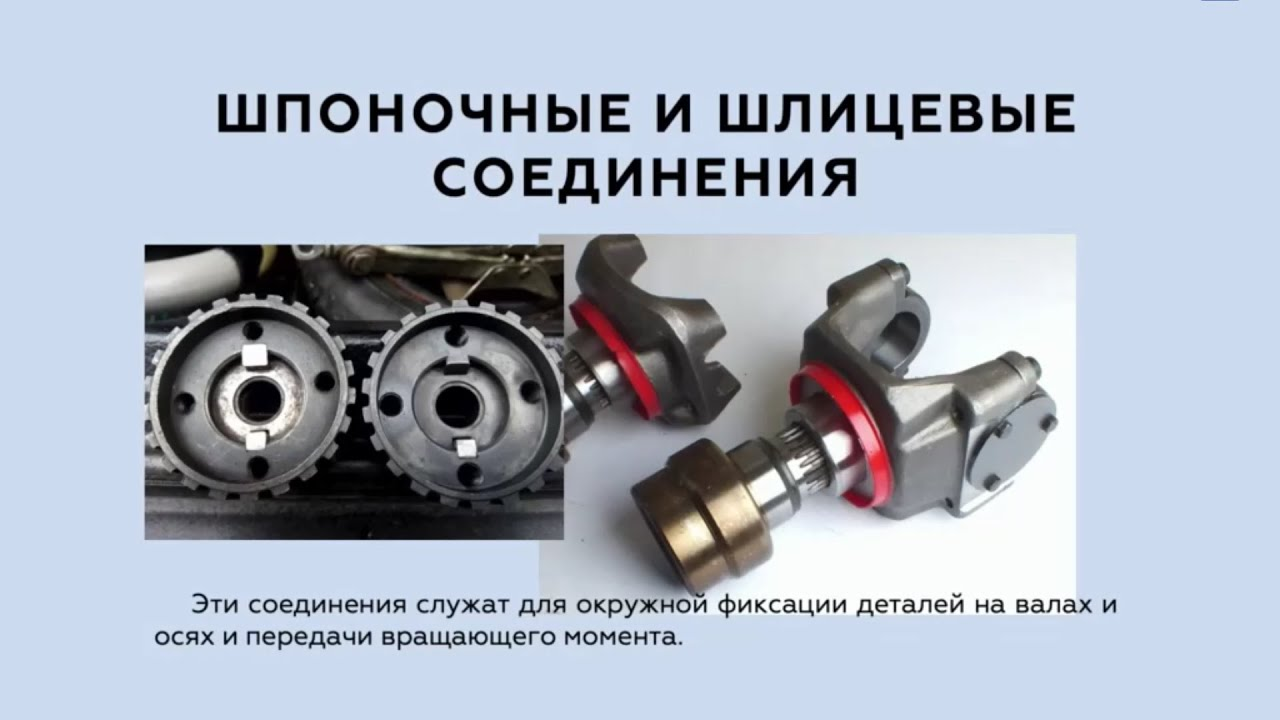
\includegraphics[height=6cm,width=1\textwidth,keepaspectratio]{key_rus_video.jpg}}
        \label{fig:key_rus_video.jpg}
    \end{figure}
\end{frame}

\begin{frame}[t]{Keyed}
\framesubtitle{Reference material}
\begin{itemize}
    \item \href{https://mechanicalland.com/shaft-keys/}{Shaft Keys and Keyways; Design, Explanation Applications}
\end{itemize}
\end{frame}


\begin{frame}[t]{Pin (Штифтовое)}
    \framesubtitle{}
    \begin{columns}[T,onlytextwidth]
        \begin{column}{0.49\textwidth}
            It is a fastening element in the form of a cylindrical or tapered rod designed for a fixed connection. The pin is inserted tightly into the hole that runs through both parts, preventing their mutual displacement.
        \end{column}
        \begin{column}{0.49\textwidth}
            \begin{figure}[H]
                \centering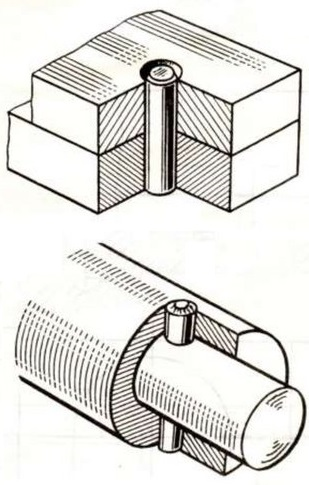
\includegraphics[height=5cm,width=1\textwidth,keepaspectratio]{stift.jpg}
                \label{fig:stift.jpg}
            \end{figure}
        \end{column}
    \end{columns}
\end{frame}

\begin{frame}[t]{Types of pin connections}
\framesubtitle{}
\vspace{-0.6cm}
    \begin{columns}[T,onlytextwidth]
        \begin{column}{0.69\textwidth}
            \begin{figure}[H]
                \begin{subfigure}{0.49\textwidth}
                    \centering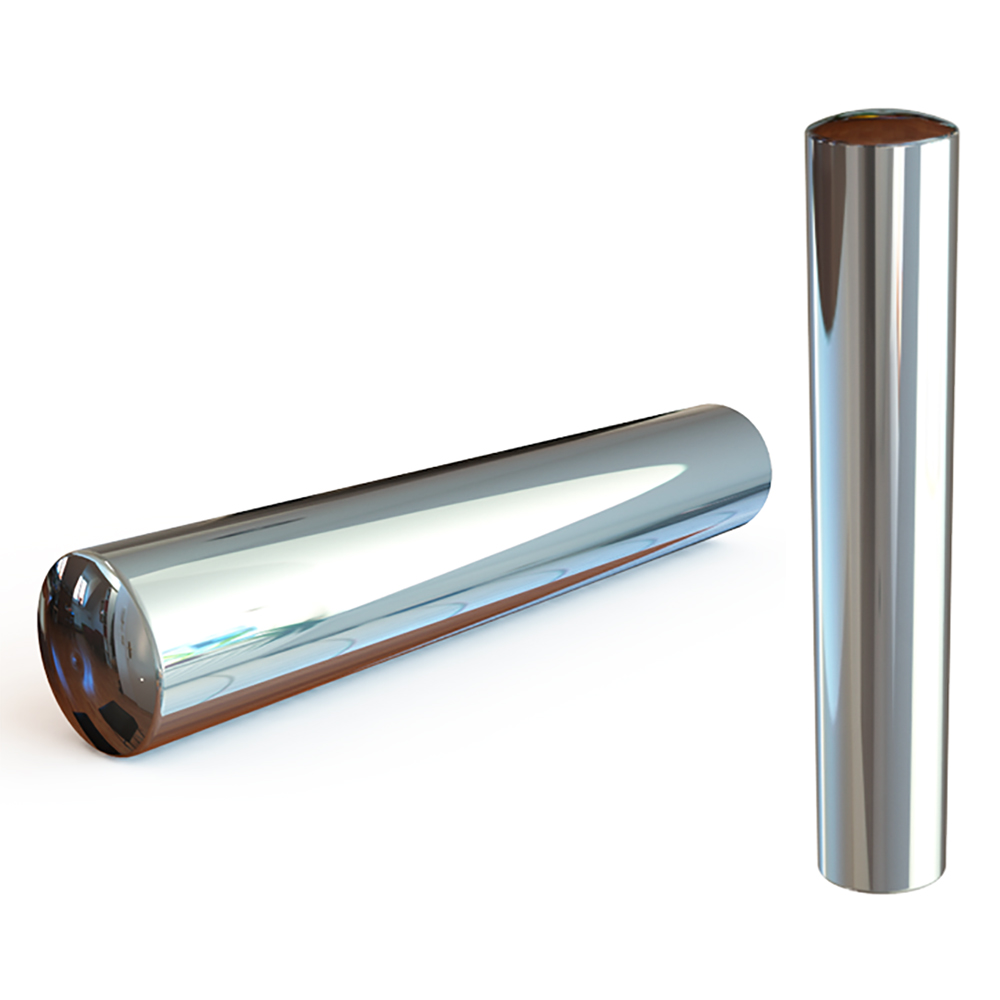
\includegraphics[height=3cm,width=1\textwidth,keepaspectratio]{pin_1.png}
                    % \caption{capture1}
                    \label{fig:pin_1.png}
                \end{subfigure}
                \begin{subfigure}{0.49\textwidth}
                    \centering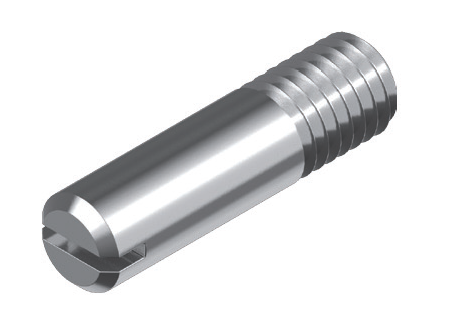
\includegraphics[height=3cm,width=1\textwidth,keepaspectratio]{pin_2.png}
                    % \caption{capture2}
                    \label{fig:pin_2.png}
                \end{subfigure}
            
                \begin{subfigure}{0.49\textwidth}
                    \centering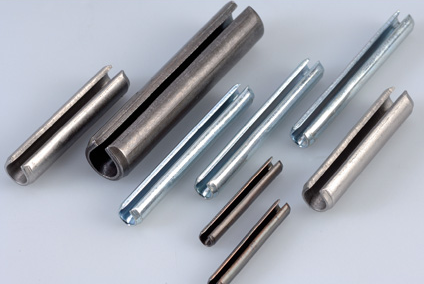
\includegraphics[height=3cm,width=1\textwidth,keepaspectratio]{pin_3.png}
                    % \caption{capture3}
                    \label{fig:pin_3.png}
                \end{subfigure}
                \begin{subfigure}{0.49\textwidth}
                    \centering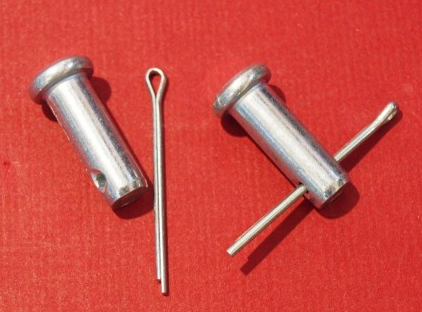
\includegraphics[height=3cm,width=1\textwidth,keepaspectratio]{pin_4.png}
                    % \caption{capture4}
                    \label{fig:pin_4.png}
                \end{subfigure}
            \end{figure}
        \end{column}
        \begin{column}{0.29\textwidth}
            \vspace{1cm}
            \begin{figure}[H]
                \centering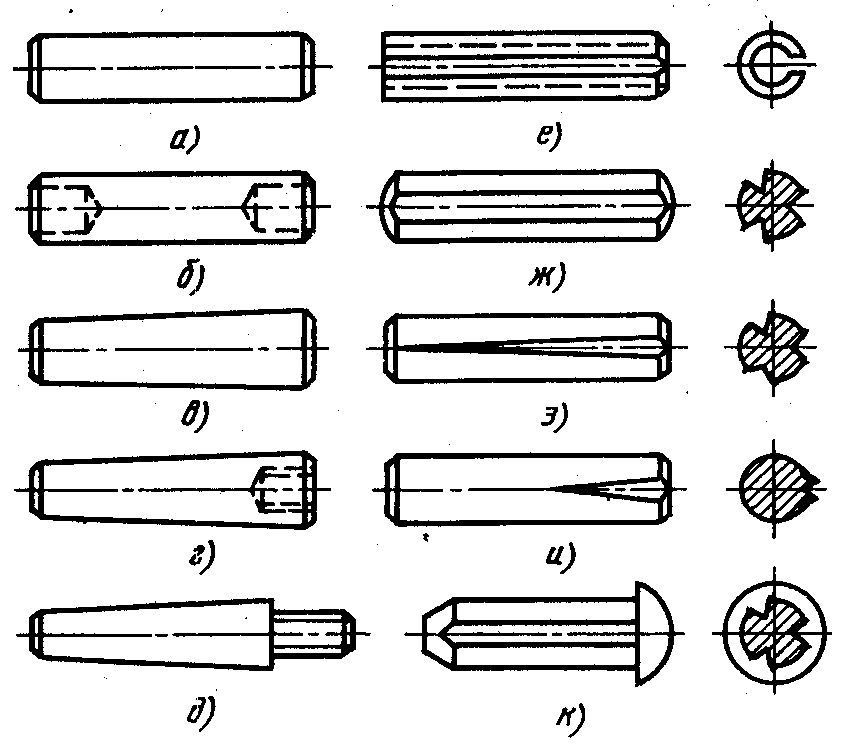
\includegraphics[height=5cm,width=1\textwidth,keepaspectratio]{types_of_pin.png}
                % \caption{caption_name}
                \label{fig:types_of_pin.png}
            \end{figure}
        \end{column}
    \end{columns}
\end{frame}

\begin{frame}[t]{Pin connection Applications}
\framesubtitle{}
\vspace{-0.6cm}
    \begin{figure}[H]
        \begin{subfigure}{0.49\textwidth}
            \centering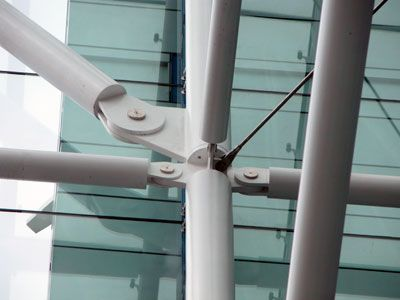
\includegraphics[height=2.5cm,width=1\textwidth,keepaspectratio]{pin_use_1.png}
            \caption*{Common usage}
            \label{fig:pin_use_1.png}
        \end{subfigure}
        \begin{subfigure}{0.49\textwidth}
            \centering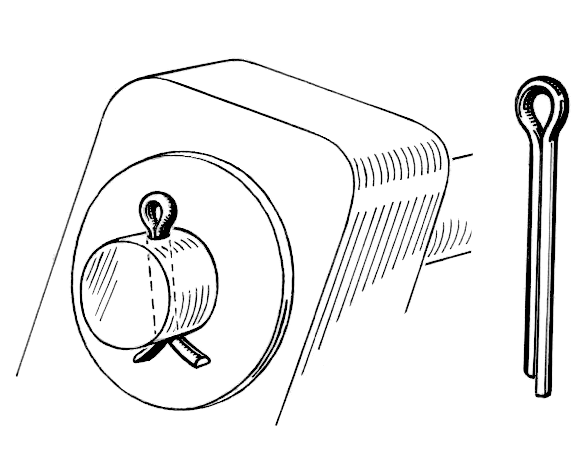
\includegraphics[height=2.5cm,width=1\textwidth,keepaspectratio]{pin_use_2.png}
            \caption*{Splint pin (шплинтовое)}
            \label{fig:pin_use_2.png}
        \end{subfigure}
    
        \begin{subfigure}{0.49\textwidth}
            \centering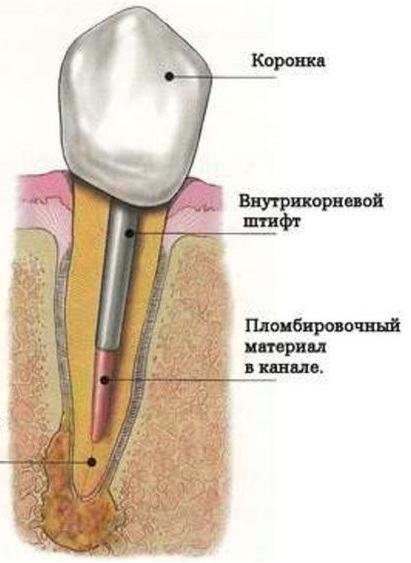
\includegraphics[height=2.5cm,width=1\textwidth,keepaspectratio]{pin_use_3.jpg}
            \caption*{Stomatology}
            \label{fig:pin_use_3.jpg}
        \end{subfigure}
        \begin{subfigure}{0.49\textwidth}
            \centering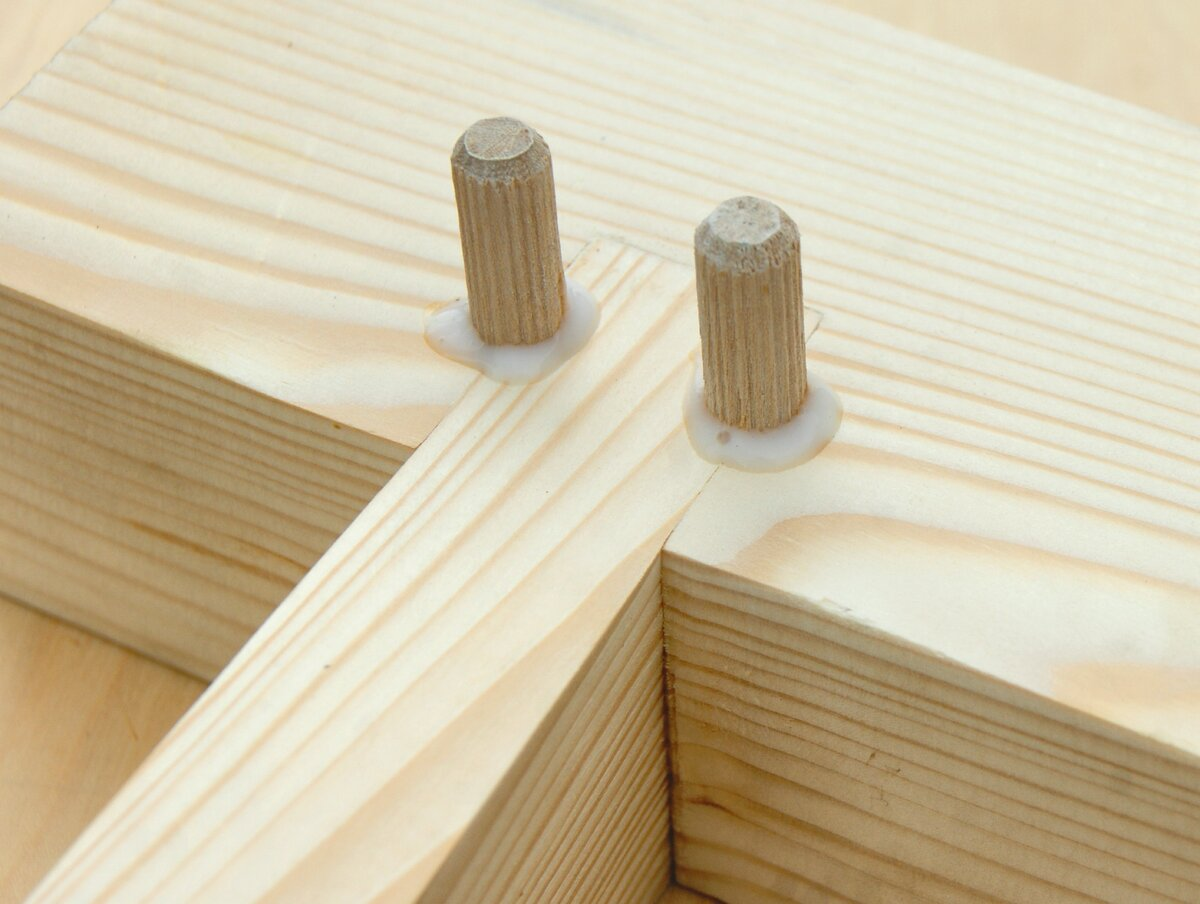
\includegraphics[height=2.5cm,width=1\textwidth,keepaspectratio]{dowel.jpeg}
            \caption*{Dowel (шкант)}
            \label{fig:dowel.jpeg}
        \end{subfigure}
    \end{figure}
\end{frame}

\begin{frame}[t]{Pin types}
    \framesubtitle{Video}
    \vspace{-0.6cm}
    \begin{figure}[H]
        \href{https://youtu.be/W-0ZV9zXpc0}{
            \centering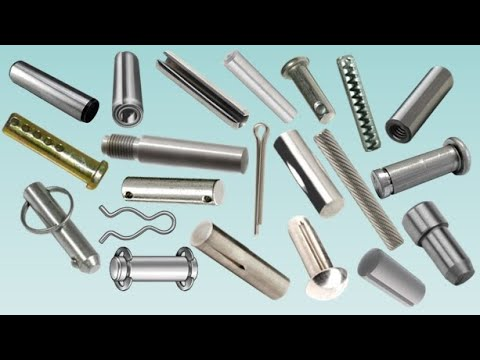
\includegraphics[height=6cm,width=1\textwidth,keepaspectratio]{pin_types_video.jpg}}
        \label{fig:pin_types_video.jpg}
    \end{figure}
\end{frame}

\begin{frame}[t]{Split Pin (шплинтовое)}
    \framesubtitle{Video}
    \vspace{-0.6cm}
    \begin{figure}[H]
        \href{https://youtu.be/SpY0tJMY0hg}{
            \centering
\includegraphics[height=6cm,width=1\textwidth,keepaspectratio]{splint_pin_video.jpg}}
        \label{fig:splint_pin_video.jpg}
    \end{figure}
\end{frame}

\begin{frame}[t]{Threaded}
    \framesubtitle{}

\end{frame}

\begin{frame}[t]{Magic 2 sided screw}
    \framesubtitle{Video}
    \vspace{-0.6cm}
    \begin{figure}[H]
        \href{https://youtu.be/cDfMI5ahbJI?t=722}{
            \centering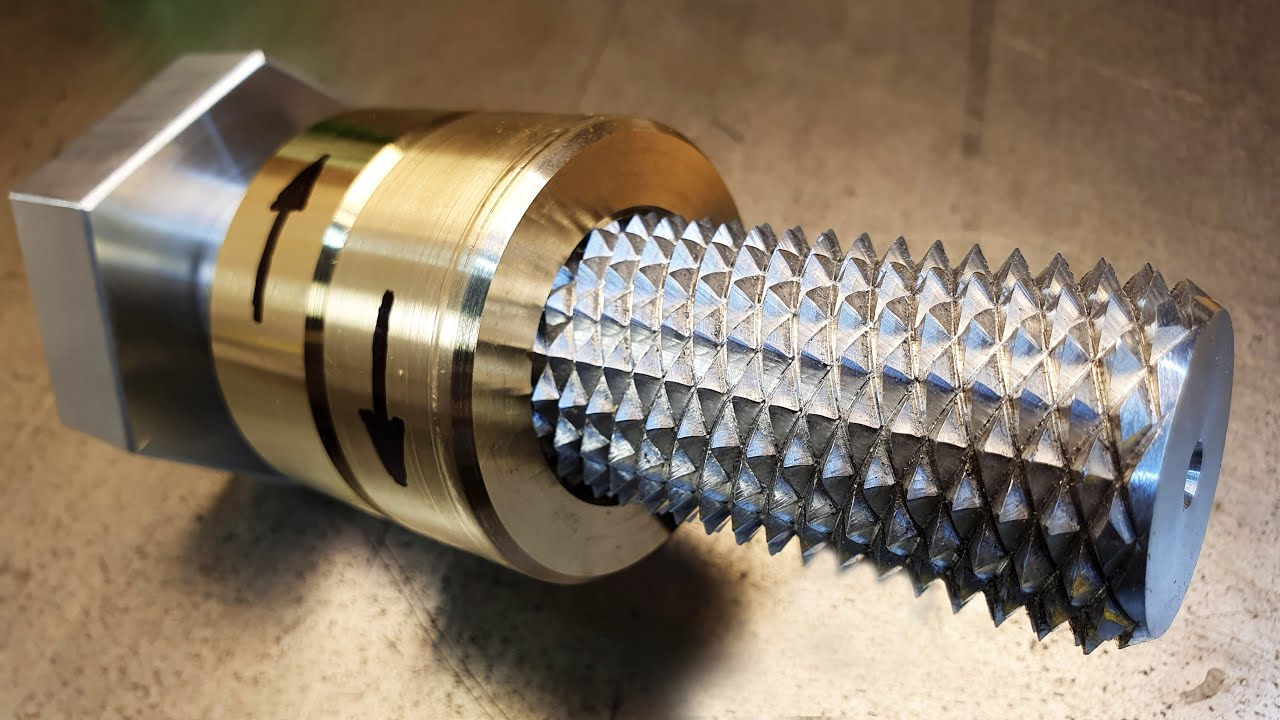
\includegraphics[height=6cm,width=1\textwidth,keepaspectratio]{two_sided_screw_video.jpg}}
        \label{fig:two_sided_screw_video.jpg}
    \end{figure}
\end{frame}

\begin{frame}[t]{Threaded}
    \framesubtitle{Reference material}
    \begin{itemize}
        \item \href{https://youtu.be/LYUKs4LePc4}{Threaded connection (video, rus)}
    \end{itemize}
    \end{frame}

\begin{frame}[t]{Glued}
    \framesubtitle{}

\end{frame}

\begin{frame}[t]{Riveting}
    \framesubtitle{}

\end{frame}

\begin{frame}[t]{Riveting rus}
    \framesubtitle{Video}
    \vspace{-0.6cm}
    \begin{figure}[H]
        \href{https://youtu.be/H7ssVv_MtNQ}{
            \centering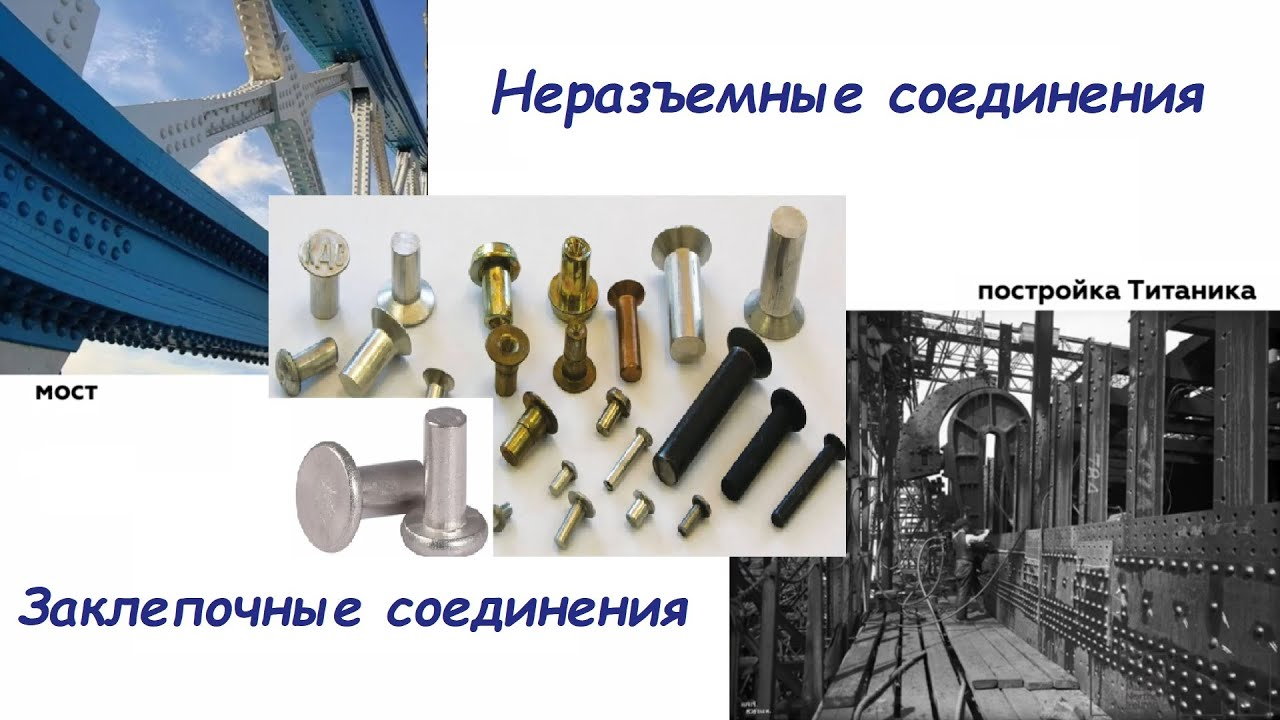
\includegraphics[height=6cm,width=1\textwidth,keepaspectratio]{riveting_rus_video.jpg}}
        \label{fig:riveting_rus_video.jpg}
    \end{figure}
\end{frame}

\begin{frame}[t]{Welding}
    \framesubtitle{}

\end{frame}

\begin{frame}[t]{Welding rus}
    \framesubtitle{Video}
    \vspace{-0.6cm}
    \begin{figure}[H]
        \href{https://youtu.be/bCe_WB7vO-A}{
            \centering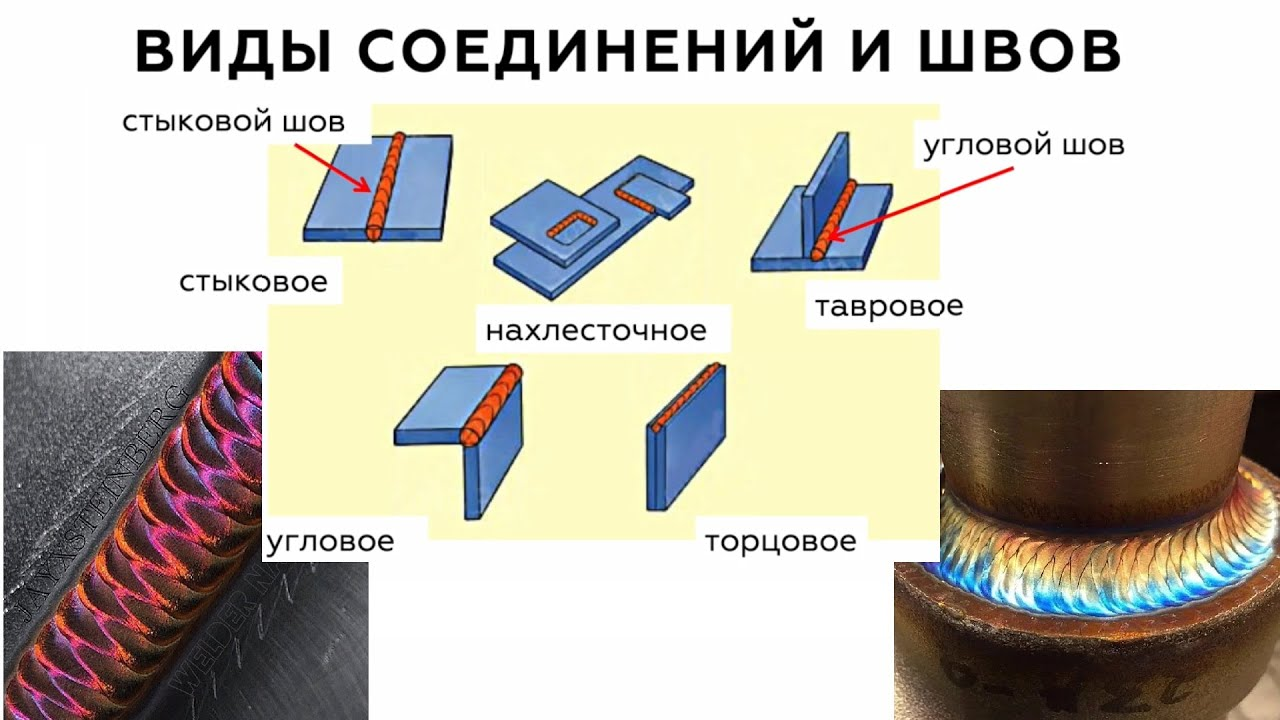
\includegraphics[height=6cm,width=1\textwidth,keepaspectratio]{welding_rus_video.jpg}}
        \label{fig:welding_rus_video.jpg}
    \end{figure}
\end{frame}

\begin{frame}[t]{Difference between Soldering and Brazing}
    \framesubtitle{Video}
    \vspace{-0.6cm}
    \begin{figure}[H]
        \href{https://youtu.be/Rq_Vuye4HL0}{
            \centering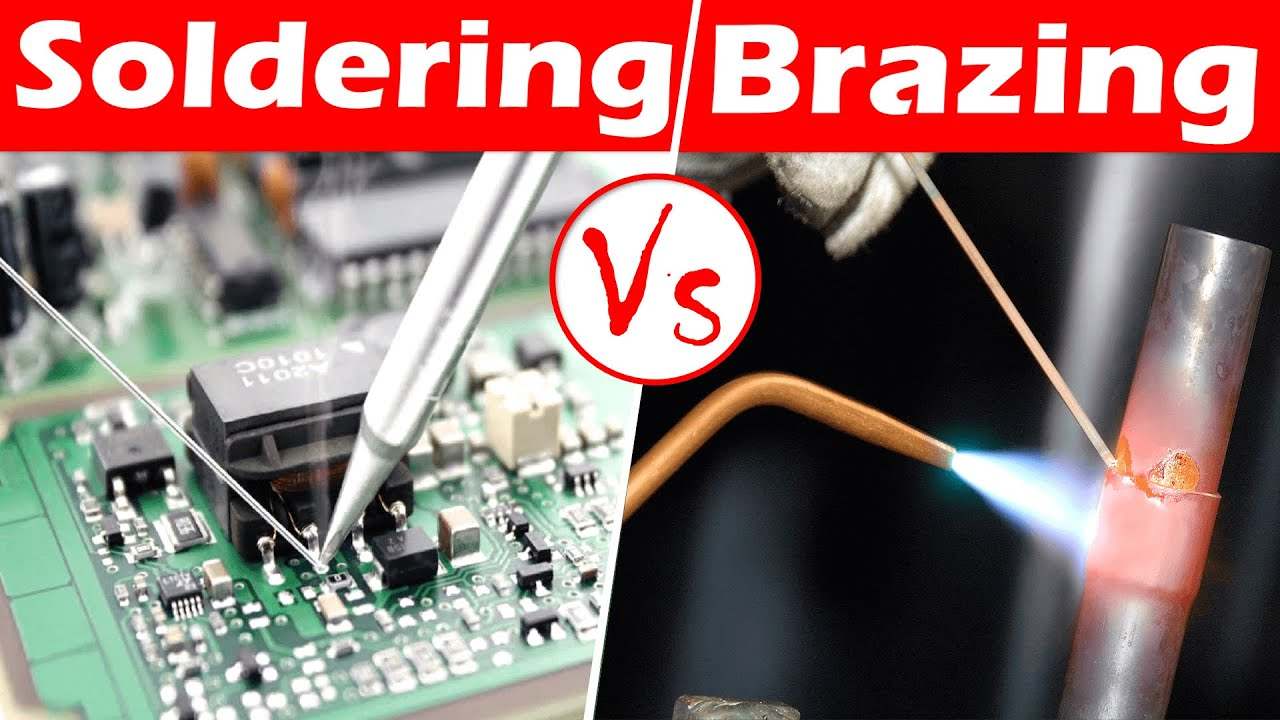
\includegraphics[height=6cm,width=1\textwidth,keepaspectratio]{dif_sold_braz_video.jpg}}
        \label{fig:dif_sold_braz_video.jpg}
    \end{figure}
\end{frame}

\begin{frame}[t]{Soldering}
    \framesubtitle{}

\end{frame}

\begin{frame}[t]{Reference material}
    \framesubtitle{}
    \begin{enumerate}
        \item \href{https://www.uti.edu/blog/welding/brazing-soldering-welding}{Brazing soldering welding difference}
        \item Mott R. L., Vavrek E. M., Wang J. Machine Elements in Mechanical Design, Ed. --- 2011
        \item Avallone E. A., Baumeister III T., Sadegh A. Marks' standard handbook for mechanical engineers. --- McGraw-Hill Education, 2007.
        \item Budynas R. G. et al. Shigley's mechanical engineering design. --- New York : McGraw-Hill, 2011.
        \item \href{https://youtu.be/jyun8hmWjS4}{Types of connection (rus, video)}
        \item \href{https://engineeringbookspdf.com/category/mechanical-engineering-pdf-books/}{A lot of engineering books in english}
    \end{enumerate}

    % 
\end{frame}



\fbckg{fibeamer/figs/last_page.png}
\frame[plain]{}

\end{document}